\chapter{PENGUJIAN DAN EVALUASI}
\par Bab ini membahas pengujian dan evaluasi terhadap perangkat lunak yang telah diimplementasikan, dengan menggunakan metode \textit{blackbox}.

\section{Lingkungan Pengujian}
\par Lingkungan yang digunakan untuk menguji tugas akhir ini memiliki spesifikasi perangkat keras dan lunak yang ditunjukkan pada tabel \ref{5:tabel_spesifikasi_server}, \ref{5:tabel_spesifikasi_perangkat_android}, dan \ref{5:tabel_spesifikasi_perangkat_ios}.
\begin{longtable}{|p{3cm}|p{6.5cm}|}
	\caption{Spesifikasi Server} \label{5:tabel_spesifikasi_server} \\ \hline
    \rowcolor{lightgray} Komponen & Spesifikasi \\ \hline
    CPU & Intel(R) Xeon(R) CPU E5-2690 v4 \\ \hline
    CPU Core & 4 \\ \hline
    Memory & 8 GB \\ \hline
    Sistem Operasi & Ubuntu 18.04 \\ \hline
\end{longtable}
\begin{longtable}{|p{3cm}|p{6.5cm}|}
	\caption{Spesifikasi Perangkat Android} \label{5:tabel_spesifikasi_perangkat_android} \\ \hline
	\rowcolor{lightgray} Komponen & Spesifikasi \\ \hline
    CPU & Snapdragon 636 \\ \hline
    Memory & 3 GB \\ \hline
    Sistem Operasi & Android 9 (Pie) \\ \hline
\end{longtable}
\begin{longtable}{|p{3cm}|p{6.5cm}|}
	\caption{Spesifikasi Perangkat iOS} \label{5:tabel_spesifikasi_perangkat_ios} \\ \hline
	\rowcolor{lightgray} Komponen & Spesifikasi \\ \hline
    CPU & Apple A10 Fusion \\ \hline
    Memory & 3 GB \\ \hline
    Sistem Operasi & iOS 12 \\ \hline
\end{longtable}

\section{Pengujian Fungsional}
\par Pengujian fungsional dilakukan untuk mengetahui apakah sistem yang dibangun sudah memiliki kebutuhan fungsional yang diperlukan.

\subsection{Pengujian Pembuatan Packet}
\par Pengujian Pembuatan Packet dilakukan untuk mengetahui apakah Scheduler berhasil membuatkan data \textit{packet} dari \textit{batch} dengan tepat. Hasil uji dapat dilihat pada Tabel \ref{t:uji_pembuatan_packet}.
\begin{longtable}{|p{3cm}|p{6.5cm}|}
	\caption{Hasil Uji Pembuatan \textit{Packet}} \label{t:uji_pembuatan_packet} \\ \hline
	\textbf{Kode} & FT-01 \\ \hline
	\textbf{Nama} & Pengujian Pembuatan Packet \\ \hline
	\textbf{Tujuan} & Menguji apakah sistem mampu membuatkan data \textit{packet} dari data \textit{batch} \\ \hline
	\textbf{Kondisi Awal} & Scheduler aktif \\ \hline
	\textbf{Langkah Pengujian} &  
	\begin{enumerate}
		\item Pengguna menambahkan data \textit{batch} baru lewat halaman kirim notifikasi di modul manajemen.
		\item Setelah 30 detik, data \textit{packet} akan disimpan di sistem basis data.
	\end{enumerate} \\ \hline
	\textbf{Hasil yang diharapkan} & Data \textit{packet} tersimpan di sistem basis data \\ \hline
	\textbf{Hasil yang diperoleh} & Data \textit{packet} tersimpan di sistem basis data \\ \hline
	\textbf{Hasil pengujian} & Berhasil \\ \hline
\end{longtable}

\subsection{Pengujian Menambahkan Packet ke Antrian}
\par Pengujian menambahkan \textit{packet} dilakukan untuk mengetahui apakah Scheduler berhasil menambahkan \textit{packet} ke antrian dengan tepat. Hasil uji dapat dilihat pada Tabel \ref{t:uji_pembuatan_antrian}.
\begin{longtable}{|p{3cm}|p{6.5cm}|}
	\caption{Hasil Uji Menambahkan \textit{Packet} ke Antrian} \label{t:uji_pembuatan_antrian} \\ \hline
	\textbf{Kode} & FT-02 \\ \hline
	\textbf{Nama} & Pengujian Pembuatan Antrian \\ \hline
	\textbf{Tujuan} & Menguji apakah sistem mampu membuatkan data antrian dari data \textit{packet} \\ \hline
	\textbf{Kondisi Awal} & Scheduler aktif \\ \hline
	\textbf{Langkah Pengujian} &  
	\begin{enumerate}
		\item Pengguna menambahkan data \textit{batch} baru lewat halaman kirim notifikasi di modul manajemen.
		\item 30 detik setelah waktu pengiriman \textit{batch}, data \textit{packet} untuk \textit{batch} akan tersimpan di sistem antrian pesan.
	\end{enumerate} \\ \hline
	\textbf{Hasil yang diharapkan} & Data \textit{packet} tersimpan di sistem antrian pesan. \\ \hline
	\textbf{Hasil yang diperoleh} & Data \textit{packet} tersimpan di sistem antrian pesan. \\ \hline
	\textbf{Hasil pengujian} & Berhasil \\ \hline
\end{longtable}

\subsection{Pengujian Pengiriman Packet ke APNs}
\par Pengujian pengiriman \textit{packet} ke APNs dilakukan untuk mengetahui apakah Sender APN berhasil mengirimkan \textit{packet} ke layanan APNs dengan tepat. Hasil uji dan notifikasi dapat dilihat pada Tabel \ref{t:uji_pengiriman_packet_apn} dan Gambar \ref{f:ss_ios}.
\begin{longtable}{|p{3cm}|p{6.5cm}|}
	\caption{Hasil Uji Pengiriman \textit{Packet} ke APNs} \label{t:uji_pengiriman_packet_apn} \\ \hline
	\textbf{Kode} & FT-03 \\ \hline
	\textbf{Nama} & Pengujian Pembuatan Packet \\ \hline
	\textbf{Tujuan} & Menguji apakah sistem mampu mengirim \textit{packet} lewat layanan APNs \\ \hline
	\textbf{Kondisi Awal} & Scheduler dan Sender APN aktif \\ \hline
	\textbf{Langkah Pengujian} &  
	\begin{enumerate}
		\item Pengguna menambahkan data \textit{batch} baru untuk perangkat iOS lewat halaman kirim notifikasi di modul Manajemen.
		\item 1 menit setelah waktu pengiriman \textit{batch}, notifikasi akan diterima oleh perangkat iOS.
	\end{enumerate} \\ \hline
	\textbf{Hasil yang diharapkan} & Notifikasi diterima oleh perangkat iOS \\ \hline
	\textbf{Hasil yang diperoleh} & Notifikasi diterima oleh perangkat iOS \\ \hline
	\textbf{Hasil pengujian} & Berhasil \\ \hline
\end{longtable}
\begin{figure}[H]
	\centering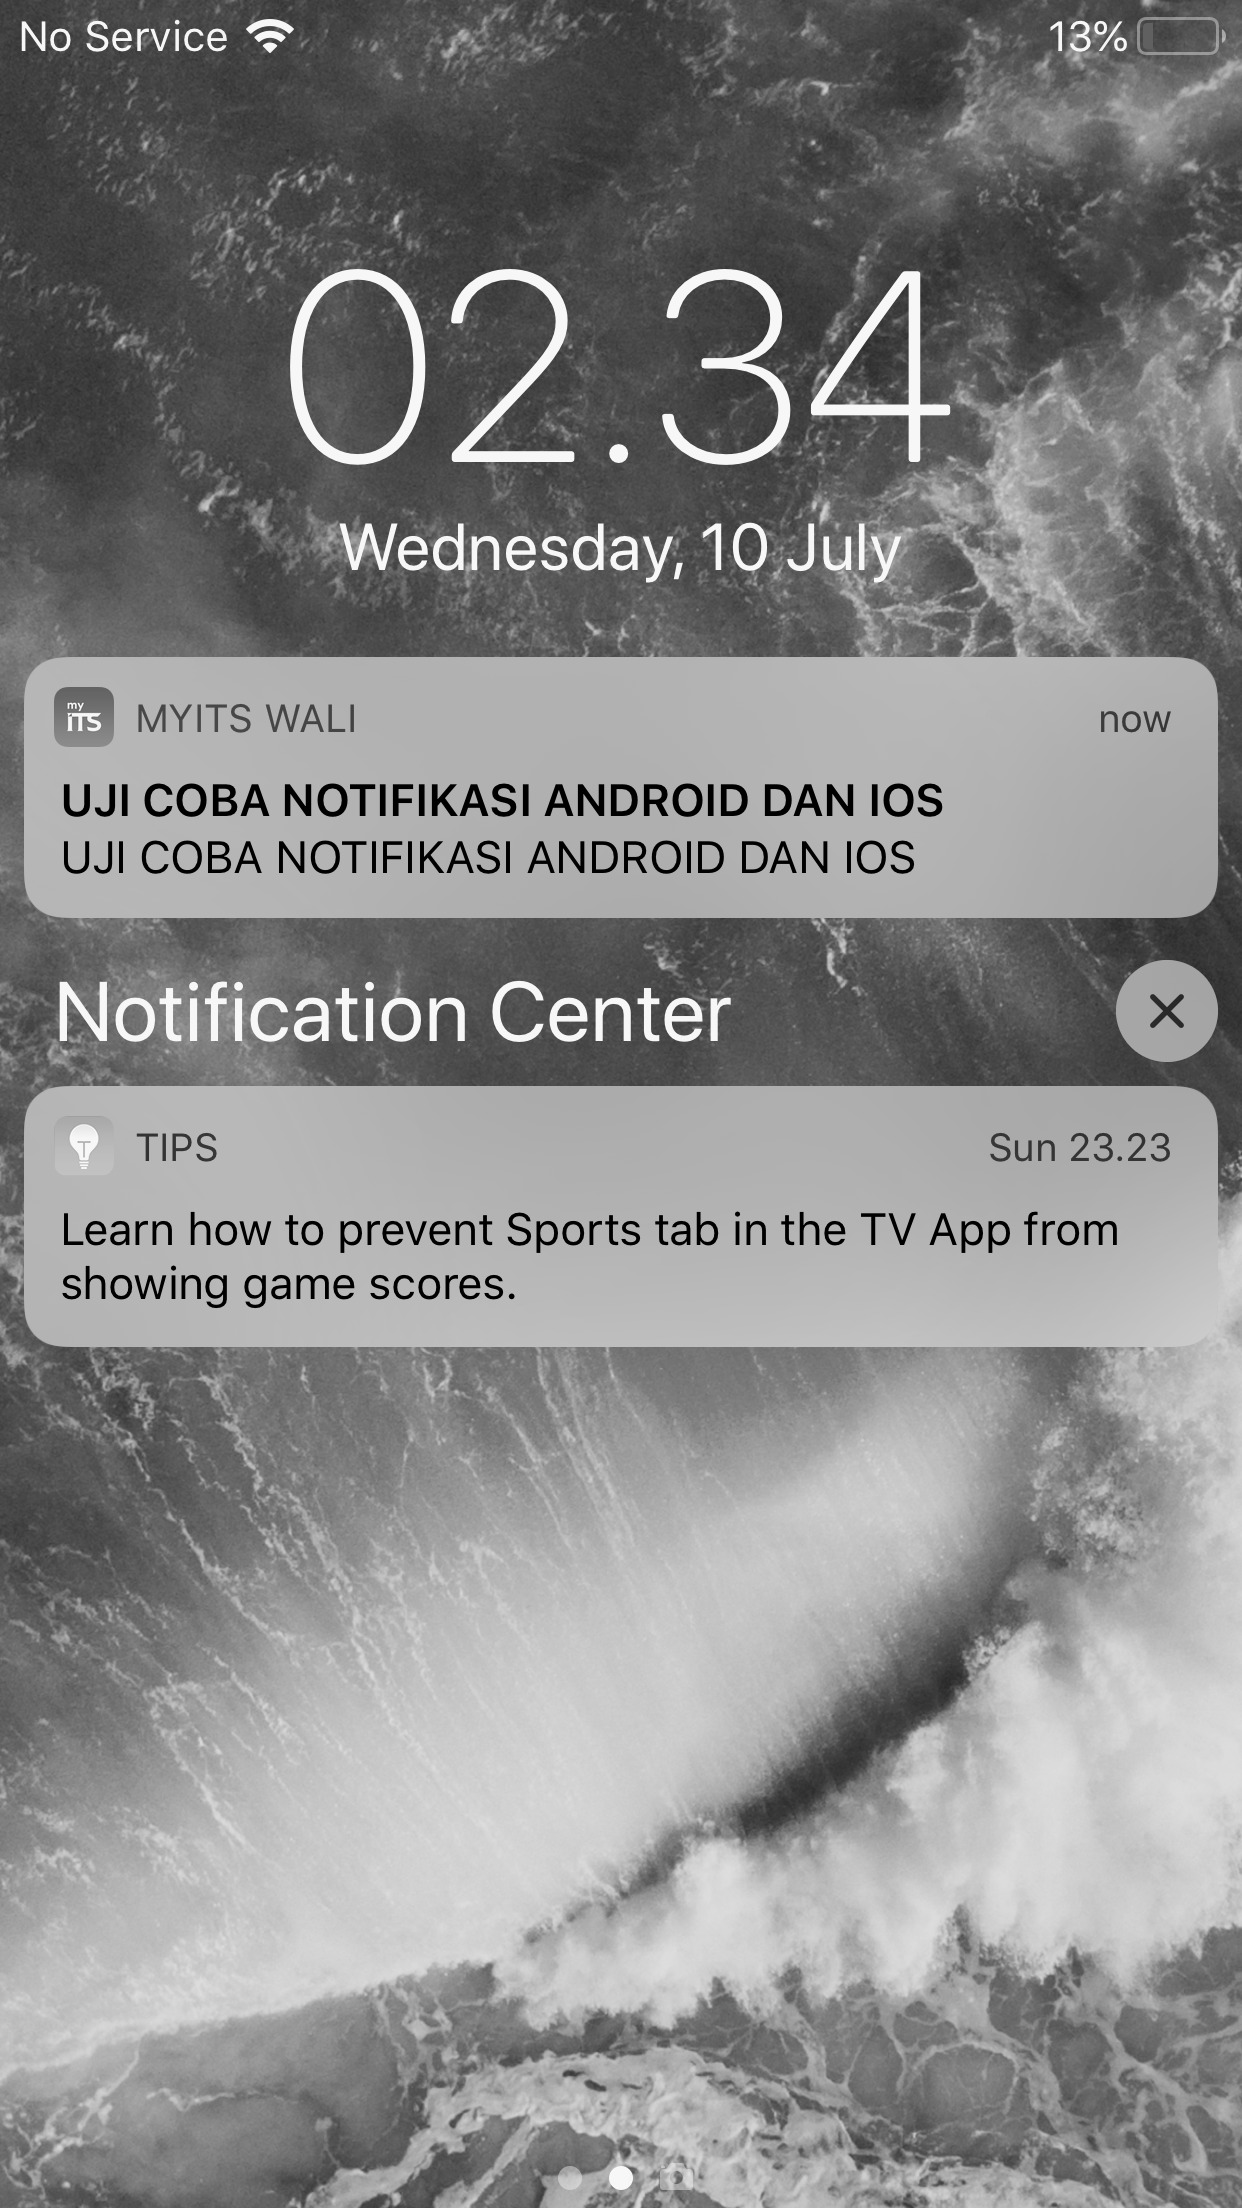
\includegraphics[width=0.5\textwidth]{bab5/figures/ss_ios.jpg}
	\caption{Hasil Notifikasi di Perangkat iOS} \label{f:ss_ios}
\end{figure}

\subsection{Pengujian Pengiriman Packet ke FCM}
\par Pengujian pengiriman \textit{packet} ke FCM dilakukan untuk mengetahui apakah Sender FCM berhasil mengirimkan \textit{packet} ke layanan FCM dengan tepat. Hasil uji dan notifikasi dapat dilihat pada Tabel \ref{t:uji_pengiriman_packet_fcm} dan Gambar \ref{f:ss_android}.
\begin{longtable}{|p{3cm}|p{6.5cm}|}
	\caption{Hasil Uji Pengiriman \textit{Packet} ke FCM} \label{t:uji_pengiriman_packet_fcm} \\ \hline
	\textbf{Kode} & FT-04 \\ \hline
	\textbf{Nama} & Pengujian Pengiriman Packet ke FCM \\ \hline
	\textbf{Tujuan} & Menguji apakah sistem mampu mengirim \textit{packet} lewat layanan FCM \\ \hline
	\textbf{Kondisi Awal} & Scheduler dan Sender FCM aktif \\ \hline
	\textbf{Langkah Pengujian} &  
	\begin{enumerate}
		\item Pengguna menambahkan data \textit{batch} baru untuk perangkat Android lewat halaman kirim notifikasi di modul Manajemen.
		\item 1 menit setelah waktu pengiriman \textit{batch}, notifikasi akan diterima oleh perangkat Android.
	\end{enumerate} \\ \hline
	\textbf{Hasil yang diharapkan} & Notifikasi diterima oleh perangkat Android \\ \hline
	\textbf{Hasil yang diperoleh} & Notifikasi diterima oleh perangkat Android \\ \hline
	\textbf{Hasil pengujian} & Berhasil \\ \hline
\end{longtable}
\begin{figure}[H]
	\centering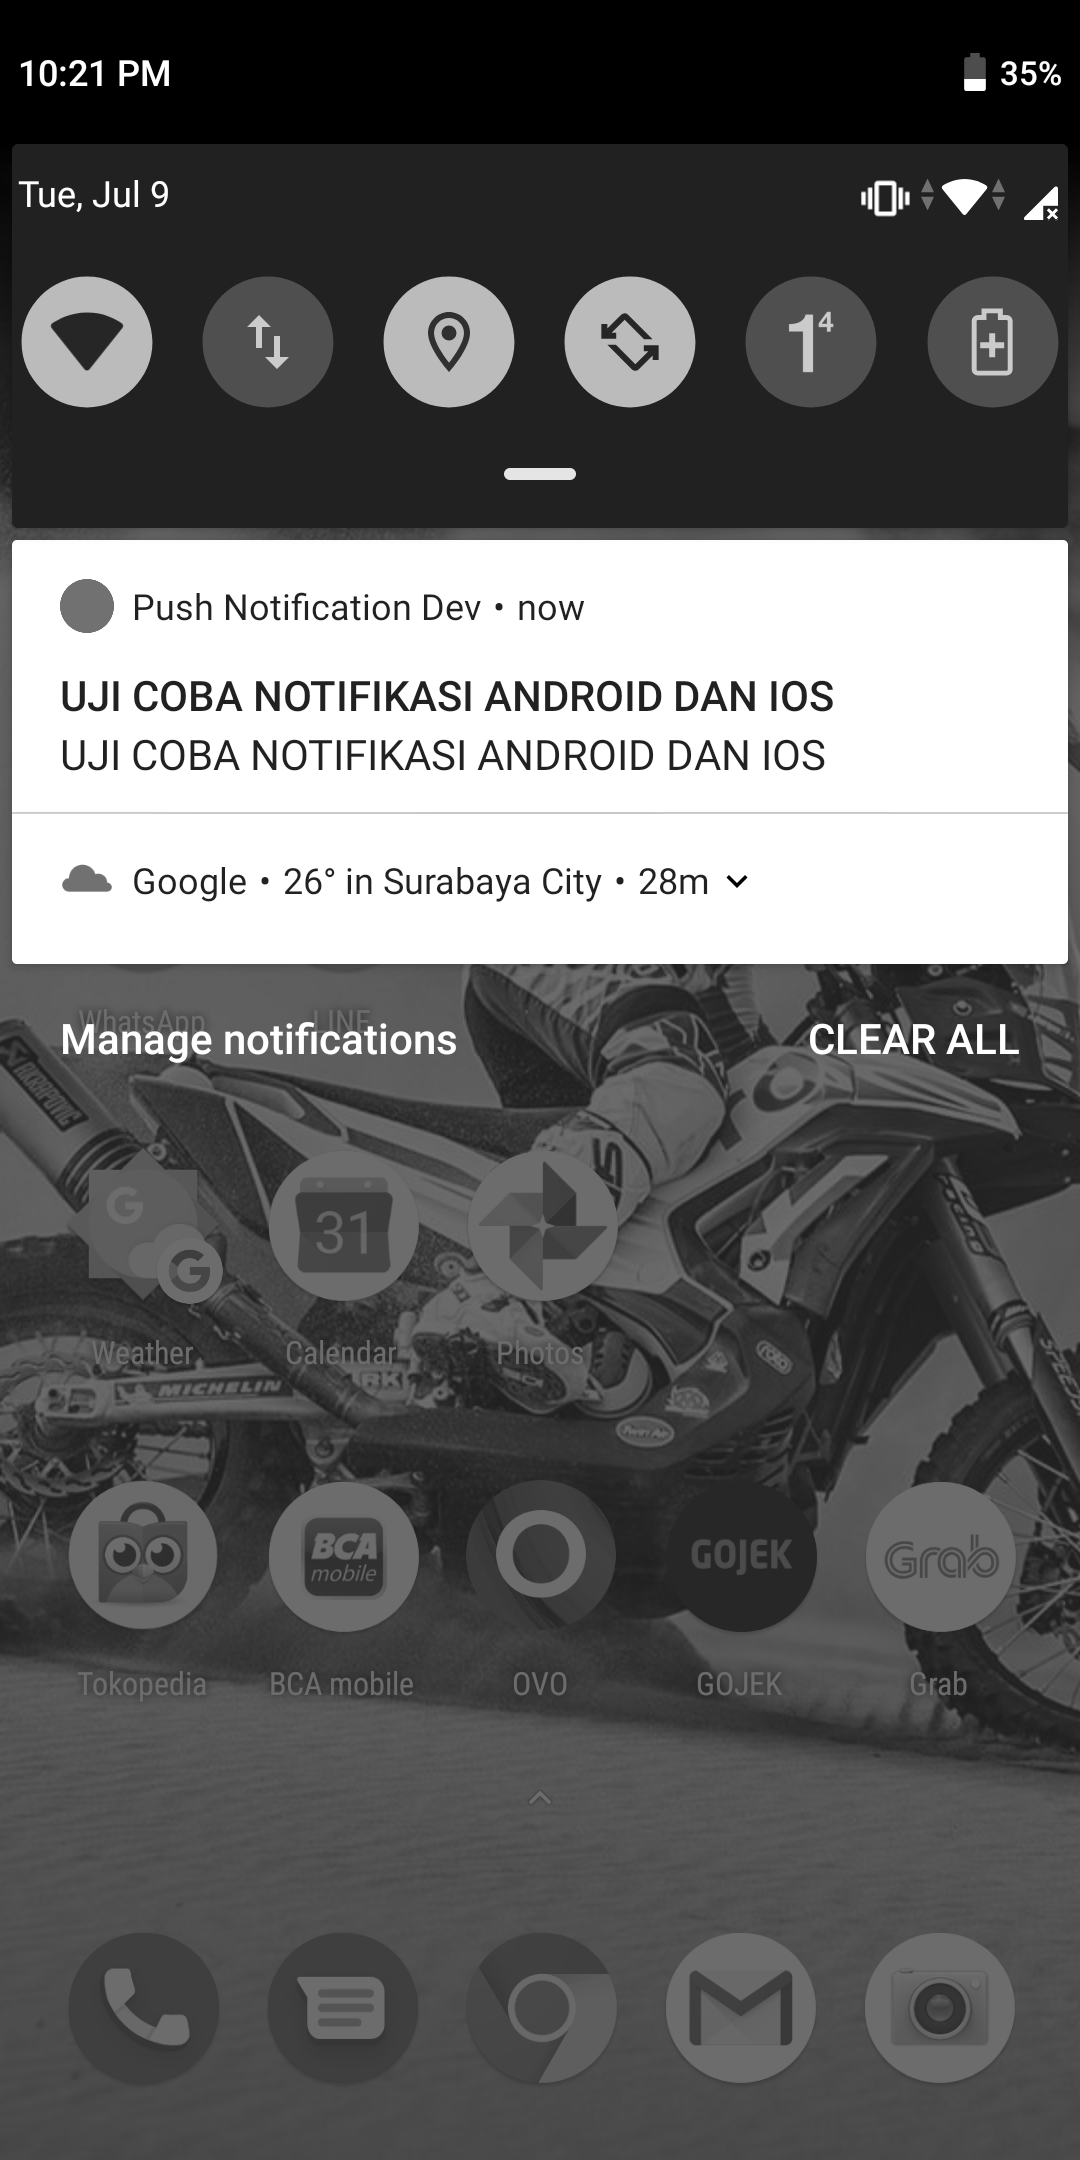
\includegraphics[width=0.5\textwidth]{bab5/figures/ss_android.png}
	\caption{Hasil Notifikasi di Perangkat Android} \label{f:ss_android}
\end{figure}

\subsection{Pengujian Menampilkan Penggunaan Sumber Daya}
\par Pengujian menampilkan penggunaan sumber daya dilakukan untuk mengetahui apakah Scheduler, Sender APN, dan Sender FCM berhasil menampilkan penggunaan sumber daya dengan tepat. Hasil uji dapat dilihat pada Tabel \ref{t:uji_menampilkan_penggunaan_sumber_daya}.
\begin{longtable}{|p{3cm}|p{6.5cm}|}
	\caption{Hasil Uji Menampilkan Penggunaan Sumber Daya} \label{t:uji_menampilkan_penggunaan_sumber_daya} \\ \hline
	\textbf{Kode} & FT-05 \\ \hline
	\textbf{Nama} & Pengujian Menampilkan Penggunaan Sumber Daya \\ \hline
	\textbf{Tujuan} & Menguji apakah sistem mampu menampilkan penggunaan sumber daya \\ \hline
	\textbf{Kondisi Awal} & Scheduler, Sender APN, dan Sender FCM aktif \\ \hline
	\textbf{Langkah Pengujian} &  
	\begin{enumerate}
		\item Pengguna mengakses \textit{endpoint} /actuator/metrics/jvm.memory.used.
		\item Sistem mengembalikan metrik penggunaan memori JVM dalam bentuk JSON.
		\item Pengguna mengakses \textit{endpoint} /actuator/metrics/system.cpu.usage.
		\item Sistem mengembalikan metrik penggunaan CPU dalam bentuk JSON.
	\end{enumerate} \\ \hline
	\textbf{Hasil yang diharapkan} & Aplikasi menampilkan metrik penggunaan Memori dan CPU \\ \hline
	\textbf{Hasil yang diperoleh} & Aplikasi menampilkan metrik penggunaan Memori dan CPU \\ \hline
	\textbf{Hasil pengujian} & Berhasil \\ \hline
\end{longtable}

\subsection{Pengujian Menampilkan Status Kesehatan}
\par Pengujian menampilkan status kesehatan dilakukan untuk mengetahui apakah Scheduler, Sender APN, dan Sender FCM berhasil menampilkan status kesehatan dengan tepat. Hasil uji dapat dilihat pada Tabel \ref{t:uji_menampilkan_status_kesehatan}.
\begin{longtable}{|p{3cm}|p{6.5cm}|}
	\caption{Hasil Uji Menampilkan Status Kesehatan} \label{t:uji_menampilkan_status_kesehatan} \\ \hline
	\textbf{Kode} & FT-06 \\ \hline
	\textbf{Nama} & Pengujian Menampilkan Status Kesehatan \\ \hline
	\textbf{Tujuan} & Menguji apakah sistem mampu menampilkan status kesehatan \\ \hline
	\textbf{Kondisi Awal} & Scheduler, Sender APN, dan Sender FCM aktif \\ \hline
	\textbf{Langkah Pengujian} &  
	\begin{enumerate}
		\item Pengguna mengakses \textit{endpoint} /actuator/health.
		\item Sistem mengembalikan metrik kesehatan layanan sistem basis data dan antrian pesan dalam bentuk JSON.
	\end{enumerate} \\ \hline
	\textbf{Hasil yang diharapkan} & Sistem menampilkan status kesehatan sistem basis data dan antrian pesan \\ \hline
	\textbf{Hasil yang diperoleh} & Sistem menampilkan status kesehatan sistem basis data dan antrian pesan \\ \hline
	\textbf{Hasil pengujian} & Berhasil \\ \hline
\end{longtable}

\subsection{Pengujian Menampilkan Konfigurasi}
\par Pengujian menampilkan konfigurasi dilakukan untuk mengetahui apakah Scheduler, Sender APN, dan Sender FCM berhasil menampilkan konfigurasi dengan tepat. Hasil uji dapat dilihat pada Tabel \ref{t:uji_menampilkan_konfigurasi}.
\begin{longtable}{|p{3cm}|p{6.5cm}|}
	\caption{Hasil Uji Menampilkan Konfigurasi} \label{t:uji_menampilkan_konfigurasi} \\ \hline
	\textbf{Kode} & FT-07 \\ \hline
	\textbf{Nama} & Pengujian Menampilkan Konfigurasi \\ \hline
	\textbf{Tujuan} & Menguji apakah sistem mampu menampilkan konfigurasi \\ \hline
	\textbf{Kondisi Awal} & Scheduler, Sender APN, dan Sender FCM aktif \\ \hline
	\textbf{Langkah Pengujian} &  
	\begin{enumerate}
		\item Pengguna mengakses \textit{endpoint} /actuator/env.
		\item Sistem mengembalikan konfigurasi sistem dalam bentuk JSON.
	\end{enumerate} \\ \hline
	\textbf{Hasil yang diharapkan} & Sistem menampilkan konfigurasi yang digunakan \\ \hline
	\textbf{Hasil yang diperoleh} & Sistem menampilkan konfigurasi yang digunakan \\ \hline
	\textbf{Hasil pengujian} & Berhasil \\ \hline
\end{longtable}

\subsection{Pengujian Menampilkan Log}
\par Pengujian menampilkan \textit{log} dilakukan untuk mengetahui apakah Scheduler, Sender APN, dan Sender FCM berhasil menampilkan \textit{log} dengan tepat. Hasil uji dapat dilihat pada Tabel \ref{t:uji_menampilkan_log}.
\begin{longtable}{|p{3cm}|p{6.5cm}|}
	\caption{Hasil Uji Menampilkan \textit{Log}} \label{t:uji_menampilkan_log} \\ \hline
	\textbf{Kode} & FT-08 \\ \hline
	\textbf{Nama} & Pengujian Menampilkan \textit{Log} \\ \hline
	\textbf{Tujuan} & Menguji apakah sistem mampu menampilkan \textit{log} \\ \hline
	\textbf{Kondisi Awal} & Scheduler, Sender APN, dan Sender FCM aktif \\ \hline
	\textbf{Langkah Pengujian} &  
	\begin{enumerate}
		\item Pengguna mengakses \textit{endpoint} /actuator/logfile.
		\item Sistem mengembalikan isi \textit{log} sistem bentuk teks.
	\end{enumerate} \\ \hline
	\textbf{Hasil yang diharapkan} & Sistem menampilkan isi \textit{log} \\ \hline
	\textbf{Hasil yang diperoleh} & Sistem menampilkan isi \textit{log} \\ \hline
	\textbf{Hasil pengujian} & Berhasil \\ \hline
\end{longtable}

\section{Pengujian Non Fungsional}
\par Pengujian non fungsional dilakukan untuk mengetahui apakah sistem yang dibangun sudah memenuhi kebutuhan non fungsional yang diperlukan.

\subsection{Pengujian Performa}
\par Pengujian performa dilakukan untuk mengetahui seberapa cepat sistem dalam mengirim \textit{packet} ke layanan APNs dan FCM. Hasil uji dapat dilihat pada Tabel \ref{t:performa}.
\begin{longtable}{|p{1.3cm}|p{1.3cm}|p{1.3cm}|p{1.8cm}|p{1.8cm}|p{1.8cm}|}
	\caption{Hasil Uji Performa Pengiriman \textit{Packet}} \label{t:performa} \\ \hline
	\rowcolor{lightgray} & \multicolumn{2}{c|}{Jumlah Perangkat} & \multicolumn{3}{c|}{Waktu Pengolahan \textit{Packet}} \\ \hhline{~|*5{-}|}
	\rowcolor{lightgray} \multirow{-2}{*}{Kode} & iOS & Android & Pembuatan & Pengiriman & Total \\ \hline
	NFT-01 & 1.000 & 1.000 & 00:00:04 & 00:02:13 & 00:02:17 \\ \hline
	NFT-02 & 10.000 & 10.000 & 00:00:25 & 00:12:09 & 00:12:34 \\ \hline
	NFT-03 & 100.000 & 100.000 & 00:03:46 & 01:57:46 & 02:01:32 \\ \hline
\end{longtable}

\subsection{Pengujian Keandalan}
\par Pengujian keandalan dilakukan untuk mengetahui tingkat keberhasilan pengiriman \textit{packet} ke perangkat pengguna.

\subsubsection{Pengujian Keandalan Pengiriman Packet ke Perangkat iOS}
\par Pengujian keandalan pengiriman \textit{packet} ke perangkat iOS dilakukan untuk mengetahui tingkat keberhasilan pengiriman \textit{packet} ke layanan APNs dan perangkat iOS. Hasil uji dapat dilihat pada Tabel \ref{t:keandalan_ios}, dan analisis kegagalan pada Tabel \ref{t:analisis_ios}.
\begin{longtable}{|p{1.3cm}|p{3cm}|p{2cm}|p{2cm}|}
	\caption{Hasil Uji Keandalan Pengiriman \textit{Packet} ke Perangkat iOS} \label{t:keandalan_ios} \\ \hline
	\rowcolor{lightgray} &  & \multicolumn{2}{c|}{Jumlah Packet Diterima} \\ \hhline{~|~|*2{-}|}
	\rowcolor{lightgray} \multirow{-2}{*}{Kode} & \multirow{-2}{*}{Jumlah Perangkat} & APNs & iOS \\ \hline
	NFT-04 & 1.000 & 1.000 & 1.000 \\ \hline
	NFT-05 & 10.000 & 10.000 & 9.984 \\ \hline
	NFT-06 & 100.000 & 100.000 & 99.848 \\ \hline
\end{longtable}
\begin{longtable}{|p{1.3cm}|p{3cm}|p{1cm}|p{3cm}|}
	\caption{Analisis Kegagalan pada Hasil Uji Keandalan Pengiriman \textit{Packet} ke Perangkat iOS} \label{t:analisis_ios} \\ \hline
	\rowcolor{lightgray} Kode & \textit{Error} & Jumlah & Penyebab \\ \hline
	NFT-05 & TooManyRequests & 16 & \textit{Request} diblokir oleh APNs karena terlalu banyak mengirim notifikasi ke satu perangkat \\ \hline
	NFT-06 & TooManyRequests & 152 & \textit{Request} diblokir oleh APNs karena terlalu banyak mengirim notifikasi ke satu perangkat \\ \hline
\end{longtable}

\subsubsection{Pengujian Keandalan Pengiriman Packet ke Perangkat Android}
\par Pengujian keandalan pengiriman packet ke perangkat android dilakukan untuk mengetahui tingkat keberhasilan sistem dalam mengirim \textit{packet} ke layanan FCM dan perangkat Android yang digunakan untuk pengujian. Hasil uji dapat dilihat pada Tabel \ref{t:keandalan_android}.
\begin{longtable}{|p{1.3cm}|p{3cm}|p{1.5cm}|p{1.5cm}|}
	\caption{Hasil Uji Keandalan Pengiriman \textit{Packet} ke Perangkat Android} \label{t:keandalan_android} \\ \hline
	\rowcolor{lightgray} &  & \multicolumn{2}{c|}{Packet Diterima} \\ \hhline{~|~|*2{-}|}
	\rowcolor{lightgray} \multirow{-2}{*}{Kode} & \multirow{-2}{*}{Jumlah Perangkat} & FCM & Android \\ \hline
	NFT-07 & 1.000 & 1.000 & 1.000 \\ \hline
	NFT-08 & 10.000 & 10.000 & 10.000 \\ \hline
	NFT-09 & 100.000 & 100.000 & 100.000 \\ \hline
\end{longtable}

\subsection{Pengujian Ketersediaan}
\par Pengujian ketersediaan dilakukan untuk mengetahui apakah sistem tetap bekerja normal saat sedang mengirimkan \textit{packet} dalam jumlah besar. Hasil uji dapat dilihat pada tabel \ref{t:ketersediaan}.
\begin{longtable}{|p{1.3cm}|p{2.2cm}|p{1.5cm}|p{1.5cm}|p{1.5cm}|}
	\caption{Hasil Uji Ketersediaan Layanan} \label{t:ketersediaan} \\ \hline
	\rowcolor{lightgray} & & \multicolumn{3}{c|}{\textit{Downtime}} \\ \hhline{~|~|*3{-}|}
	\rowcolor{lightgray} \multirow{-2}{*}{Kode} & \multirow{-2}{*}{Jumlah Packet} & Scheduler & Sender APN & Sender FCM \\ \hline
	NFT-10 & 2.000 & - & - & - \\ \hline
	NFT-11 & 20.000 & - & - & - \\ \hline
	NFT-12 & 200.000 & - & - & - \\ \hline
\end{longtable}

\subsection{Pengujian Durabilitas}
\par Pengujian durabilitas dilakukan untuk mengetahui apakah sistem tetap bekerja normal saat salah satu layanan mati. Pengujian dibagi menjadi 2 skenario, yaitu saat Sender APN dimatikan dan Sender FCM dimatikan.

\subsubsection{Pengujian Mematikan Sementara Sender APN}
\par Pengujian mematikan sementara Sender APN dilakukan dengan cara mematikan Sender APN selama 5 menit ditengah proses pengiriman \textit{packet}. Hasil uji dapat dilihat pada Tabel \ref{t:nft_sender_apn_mati}.
\begin{longtable}{|p{3cm}|p{6.5cm}|}
	\caption{Hasil Uji Mematikan Sementara Sender APN} \label{t:nft_sender_apn_mati} \\ \hline
	\textbf{Kode} & NFT-13 \\ \hline
	\textbf{Nama} & Pengujian Mematikan Sementara Sender APN \\ \hline
	\textbf{Tujuan} & Mengetahui apakah sistem mampu mengirimkan \textit{push notification} jika Sender APN mati sementara \\ \hline
	\textbf{Kondisi Awal} & Sistem dalam keadaan berjalan \\ \hline
	\textbf{Langkah Pengujian} &  
	\begin{enumerate}
		\item Aktor membuat \textit{batch} baru lewat halaman kirim notifikasi pada modul manajemen.
		\item Sender APN dimatikan selama 5 menit.
	\end{enumerate} \\ \hline
	\textbf{Hasil yang diharapkan} & Notifikasi diterima oleh perangkat iOS \\ \hline
	\textbf{Hasil yang diperoleh} & Notifikasi diterima oleh perangkat iOS \\ \hline
	\textbf{Hasil pengujian} & Berhasil \\ \hline
\end{longtable}

\subsubsection{Pengujian Mematikan Sementara Sender FCM}
\par Pengujian mematikan sementara Sender FCM dilakukan dengan cara mematikan Sender FCM selama 5 menit ditengah proses pengiriman \textit{packet}. Hasil uji dapat dilihat pada Tabel \ref{t:nft_sender_fcm_mati}.
\begin{longtable}{|p{3cm}|p{6.5cm}|}
	\caption{Hasil Uji Mematikan Sementara Sender FCM} \label{t:nft_sender_fcm_mati} \\ \hline
	\textbf{Kode} & NFT-14 \\ \hline
	\textbf{Nama} & Pengujian Mematikan Sementara Sender FCM \\ \hline
	\textbf{Tujuan} & Mengetahui apakah sistem mampu mengirimkan \textit{push notification} jika Sender FCM mati sementara \\ \hline
	\textbf{Kondisi Awal} & Sistem dalam keadaan berjalan \\ \hline
	\textbf{Langkah Pengujian} &  
	\begin{enumerate}
		\item Aktor membuat \textit{batch} baru lewat halaman kirim notifikasi pada modul manajemen.
		\item Sender FCM dimatikan selama 5 menit.
	\end{enumerate} \\ \hline
	\textbf{Hasil yang diharapkan} & Notifikasi diterima oleh perangkat Android \\ \hline
	\textbf{Hasil yang diperoleh} & Notifikasi diterima oleh perangkat Android \\ \hline
	\textbf{Hasil pengujian} & Berhasil \\ \hline
\end{longtable}

\section{Evaluasi Hasil Pengujian}
\par Berdasarkan hasil uji, Aplikasi Push Notification Terpusat yang dibangun pada tugas akhir ini sudah memenuhi semua kebutuhan fungsional dan non fungsional yang ada. Rangkuman hasil uji untuk kebutuhan fungsional dan non fungsional dapat dilihat pada Tabel \ref{t:eval_f} dan Tabel \ref{t:eval_nf}.
\begin{longtable}{|p{1.5cm}|p{3cm}|p{1.5cm}|p{1.5cm}|}
	\caption{Rangkuman Hasil Uji Fungsional} \label{t:eval_f} \\ \hline
	\rowcolor{lightgray} Kode Kebutuhan & Nama Kebutuhan & Kode Uji & Hasil \\ \hline
	F-01 & Pembuatan \textit{Packet} & FT-01 & Berhasil \\ \hline
	F-02 & Menambahkan \textit{Packet} ke Antrian & FT-02 & Berhasil \\ \hline
	F-03 & Pengiriman \textit{Packet} ke APNs & FT-03 & Berhasil \\ \hline
	F-04 & Pengiriman \textit{Packet} ke FCM & FT-04 & Berhasil \\ \hline
	F-05 & Menampilkan Penggunaan Sumber Daya & FT-05 & Berhasil \\ \hline
	F-06 & Menampilkan Status Kesehatan & FT-06 & Berhasil \\ \hline
	F-07 & Menampilkan Konfigurasi & FT-07 & Berhasil \\ \hline
	F-08 & Menampilkan \textit{Log} & FT-08 & Berhasil \\ \hline
\end{longtable}
\begin{longtable}{|p{1.5cm}|p{2cm}|p{3cm}|p{1.5cm}|}
	\caption{Rangkuman Hasil Uji Non Fungsional} \label{t:eval_nf} \\ \hline
	\rowcolor{lightgray} Kode Kebutuhan & Aspek & Kode Uji & Hasil \\ \hline
	NF-01 & Performa & NFT-01, NFT-02, NFT-03 & Terpenuhi \\ \hline
	NF-02 & Keandalan & NFT-04, NFT-05, NFT-06, NFT-07, NFT-08, NFT-09 & Terpenuhi \\ \hline
	NF-03 & Ketersediaan & NFT-10, NFT-11, NFT-12 & Terpenuhi \\ \hline
	NF-04 & Durabilitas & NFT-13, NFT-14 & Terpenuhi \\ \hline
\end{longtable}
